\documentclass[12pt]{scrartcl}
% Schrift
%\usepackage[ngerman]{babel}
\usepackage[utf8]{inputenc}
\usepackage{courier}
\usepackage{fancyhdr}
% enable use of ö/ä/ü/ß and other unicode characters in general
%\usepackage[T1]{fontenc}

% Mathepaket
%\usepackage{amsmath,amsfonts,amssymb} 
%\usepackage{stmaryrd}


% Tabellen
\usepackage{booktabs}
\setlength{\tabcolsep}{5pt} %change column separations
\renewcommand{\arraystretch}{1.3} %change row separations

% Art der Aufzählung für enumerate
\usepackage{paralist}
\usepackage{enumitem} % für verschiedene Arten von Aufzählungen (mit Parameter label)

% Bilder einfuegen
\usepackage{graphicx}
\usepackage{subfig}

% automata drawing
\usepackage{tikz}
\usetikzlibrary{arrows, automata}

% Baume
\usepackage{qtree}

% Für Markierungen
\usepackage{color}

% handy when working together
\usepackage{todonotes}

% links and references
\usepackage{hyperref}
\usepackage{url}



\usepackage{fancyhdr}
\usepackage{url}
\usepackage{ upgreek }
\pagestyle{fancy}
\fancyhf{}
\rhead{Technical overview}
\lhead{WE App}
\rfoot{\thepage}
\usepackage{graphicx}

\title{We - A mobile App to Connect Refugees and Locals}

\begin{document}
	
\maketitle

\begin{center}
	\large \textbf{Technical overview}
\end{center}

\tableofcontents
	
\newpage
\section{Components}

The application ecosystem consists of the following main components:

\begin{itemize}
	\item a database to store all content such as user profiles, invitation details or posted messages
	\item backend server side scripts that process API calls made by the frontend (mobile apps), query the database and return datasets to the frontend
	\item an iOS app that queries the server API, stores data in its model classes and presents the data in a user interface
	\item an Android app built on the same internal model as the iOS version, using an Android adjusted user interface
	
\end{itemize}

Technologies used are:

\begin{itemize}
	\item SQL database
	\item server side PHP scripts providing an HTTP POST API and accessing the database using SQL queries
	\item iOS app written in Swift using Xcode IDE
	\item Android app written in Java using Android Studio IDE
	\item communication via XML data sets returned by the server scripts
\end{itemize}

\subsection{Entities}

The main entities that mirror specifications and are used throughout all components are:

\begin{itemize}
	\item \emph{User}: profile (email, password, age, nationality etc.), associated invitations, messages etc.
	\item \emph{Invitation}: information like description, date and time or location, associated users (owner, participants), messages (each invitation containing a public and a private chat) and join requests
	\item \emph{JoinRequest}: information about which user wants to participate in which invitation and with how many persons (single, family etc.), each join requests contains a private chat
	\item \emph{Message}: text message and timestamp with associated author, invitation and join request
\end{itemize}

\newpage
\section{Server}

The server side components consist of an SQL database and PHP scripts.

\subsection{Database}

The database holds \emph{User} information and details about all existing \emph{Invitations}, \emph{JoinRequests}, \emph{Messages} and more.\\
User passwords are never transferred in clear text but are only saved as hash values in the \texttt{User} table.

\begin{figure}[h]
	\begin{center}
		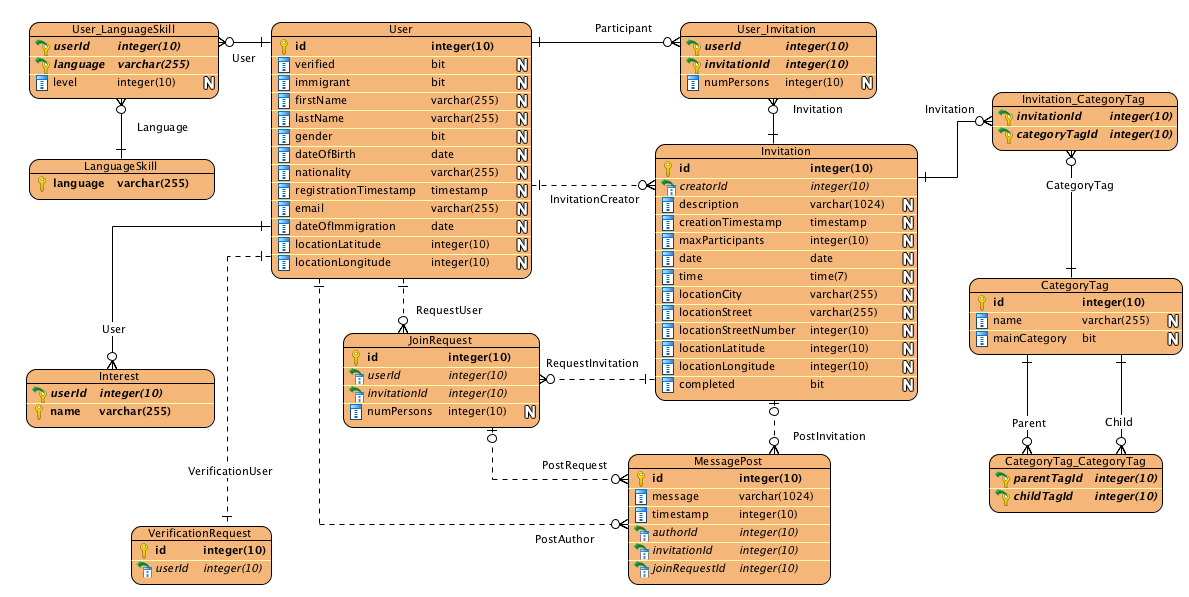
\includegraphics[width=0.9\textwidth]{../../spec/components/database_ER.png}
		\caption[Database ER diagram]{Database ER diagram}
		\label{fig:database-ER}
	\end{center}
\end{figure}

\subsection{API}

The information the frontend apps need are queried to the server API. The HTTP POST method is used to transfer data. \\
Each API call needs to specify an \texttt{action} and optional arguments. An example API call would look like this:\\
\begin{center}
	\texttt{http://<url>/API.php?action=user\_details\&user\_id=354}
\end{center}

A list of actions and required arguments is given in figures 2-4.\\

\begin{figure}
	\begin{center}
		\resizebox{\textwidth}{!}{%
		\begin{tabular}{ |c|c|c| }
			\hline
			\texttt{action} & argument & purpose \\ 
			\hline
			\texttt{user\_register} &  & registers a new user \\  
											    & \texttt{mail} & mail address (also used for login) \\  
											    & \texttt{password} & password hash value\\  
											    & \texttt{firstName} & first name \\  
											    & \texttt{lastName} & last name \\  
											    & \texttt{userType} & boolean,  immigrant or local\\  
											    & \texttt{gender} & boolean, male or female \\  
											    & \texttt{dateOfBirth} & date of birth \\  
											    & \texttt{nationality} & nationality \\  
											    & \texttt{dateOfImmigration} & date of immigration \\  
											    & \texttt{locationLatitude} & location of the user's home address \\  
												& \texttt{locationLongitude} & location of the user's home address \\  
			\hline				   
			\texttt{user\_login} & & logs in the user on the querying device \\  
												& \texttt{mail} & mail address used for login \\  
												& \texttt{password} & password hash value \\  
			\hline									
			\texttt{user\_logout} &  & logs out the user \\  
			\hline
			\texttt{user\_isLoggedIn} &  & queries whether the user is currently logged in on the querying device \\  
			\hline
			\texttt{user\_query} &  & returns a list of all users \\ 
			\hline 
			\texttt{user\_details} & & returns all user information \\  
												& \texttt{userId} & the id of the user to query details of \\ 
			\hline 
		\end{tabular}}
		\caption{available API actions and arguments for \texttt{User} queries}
		\label{fig:API-action-user}
	\end{center}
\end{figure}

\begin{figure}
	\begin{center}
		\resizebox{\textwidth}{!}{%
			\begin{tabular}{ |c|c|c| }
				\hline
				\texttt{action} & argument & purpose \\ 
				\hline
			\texttt{invitation\_create} &  & creates a new invitation \\  
												   & \texttt{name} & display name of the invitation \\   
												   & \texttt{description} & detailed description by user \\  
												   & \texttt{maxParticipants} & maximal number of participants \\ 
												   & \texttt{date} & the day the invitation is scheduled \\   
												   & \texttt{time} & the time the invitation is scheduled \\  
												   & \texttt{locationCity} & city in which the invitation is taking place \\ 
												   & \texttt{locationStreet} & street in which the invitation is taking place \\   
												   & \texttt{locationStreetNumber} & street number \\  
												   & \texttt{locationLatitude} & location of the provided address \\ 
												   & \texttt{locationLongitude} & location of the provided address \\ 
			\hline
			\texttt{invitation\_postMessage} &  & posts a message to the invitation chat \\  
												   & \texttt{invitationId} & id of the invitation \\   
												   & \texttt{message} & text message \\  
			\hline									   
			\texttt{invitation\_messages} &  & queries all messages for a given invitation \\  
												   & \texttt{invitationId} & id of the invitation \\  
			\hline									   
			\texttt{invitation\_query} &  & returns a list of invitations \\  
													& \texttt{ownerId} & only invitations by this user \\   
													& \texttt{participatingUserId} & only invitations in which this user takes part in\\  
			\hline
			\texttt{invitation\_details} &  & returns detailed information for a given invitation \\  
												   & \texttt{invitationId} & id of the invitation \\   
			\hline									   
			\texttt{invitation\_participants} &  & queries all users participating in the invitation \\  
												   & \texttt{invitationId} & id of the invitation \\   
			\hline									   
			\texttt{invitation\_delete} &  & deletes the invitation \\  
												   & \texttt{invitationId} & id of the invitation \\ 
			\hline									   
			\texttt{invitation\_update} &  & changes the invitation data \\  
												   & \texttt{invitationId} & id of the invitation \\  
												   & \texttt{...} & \emph{the same arguments as in} \texttt{invitation\_create} \emph{are used} \\   
		\hline		   
		\end{tabular}}
		\caption{available API actions and arguments for \texttt{Invitation} queries}
		\label{fig:API-action-invitation}
	\end{center}
\end{figure}												   
												   
												   
\begin{figure}
	\begin{center}
		\resizebox{\textwidth}{!}{%
			\begin{tabular}{ |c|c|c| }
				\hline
				\texttt{action} & argument & purpose \\ 
				\hline											
			\texttt{joinRequest\_create} &  & creates a new join request \\  
											& \texttt{invitationId} & id of the invitation to join in \\   
											& \texttt{userId} & id of the joining user \\  
											& \texttt{numParticipants} & number of participants joining \\ 
			\hline								
			\texttt{joinRequest\_query} &  & returns a list of join requests (TODO for user/invitaiton?) \\  
			\hline
			\texttt{joinRequest\_accept} &  & accepts a join request \\  
											& \texttt{joinRequestId} & the request's id \\   
			\hline								
			\texttt{joinRequest\_reject} &  & rejects a join request \\  
											& \texttt{joinRequestId} & the request's id \\      

			\hline
		\end{tabular}}
		\caption{Available API actions and arguments for \texttt{JoinRequest} queries}
		\label{fig:API-action-joinRequest}
	\end{center}
\end{figure}

\newpage
When receiving a query, the API script then performs the following tasks:

\begin{enumerate}
	\item read the provided \texttt{action} argument
	\item initialize a connection to the database
	\item call appropriate \texttt{processAtion} routine
	\item check if the user is logged in (except when in the \texttt{user\_login} action, where a PHP session is initiated and the variable \texttt{userId} is set which is used to check the login status)
	\item read additional arguments like \texttt{userId} or \texttt{invitaitonId}
	\item execute an SQL query that retrieves the desired information
	\item create an XML dataset an write it to the HTTP output
	
\end{enumerate}

The communication over network between the components is shown in figure 5.\\

\begin{figure}[h]
	\begin{center}
		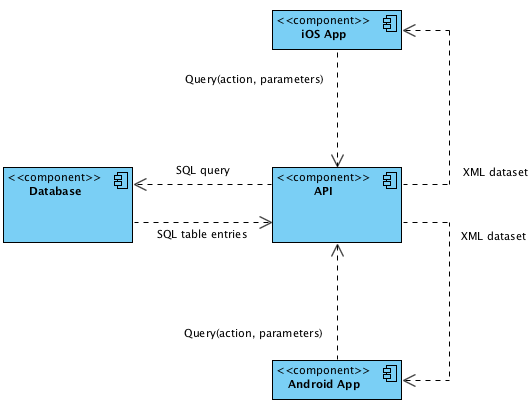
\includegraphics[width=0.9\textwidth]{../../spec/components/network_components.png}
		\caption[Component diagram of the communication over network between the app's components]{Component diagram of the communication over network between the app's components}
		\label{fig:network-component-diagram}
	\end{center}
\end{figure}

\newpage
\section{Mobile apps}

\subsection{Modules}

Both iOS and Android are built on the same frontend model using custom implementations in Swift and Java. The model is spread into the two groups \emph{Model} and \emph{Network} in XCode/Android Studio. \\
The modules in the Android app are the same as in the iOS version. For synchronous development of the two frontends it is crucial that classes and members mirror the UML specification provided in figure \ref{fig:ios-class-diagram} and are named in the same way in both iOS and Android.
\begin{itemize}
	\item 
	The \emph{Model} group contains classes like \texttt{User} or \texttt{Invitation} that mirror the entities in the database.
	
	\item
	The \emph{Network} group provides the \texttt{Query} class which is capable of sending a HTTP POST request to the server. There are a number of \texttt{Query} subclasses, one for each \texttt{action} that can be sent to the server. 
	
\end{itemize}

 The model classes make use of these \texttt{Query} subclasses to query the information they need from the server.

\begin{figure}[h]
	\begin{center}
		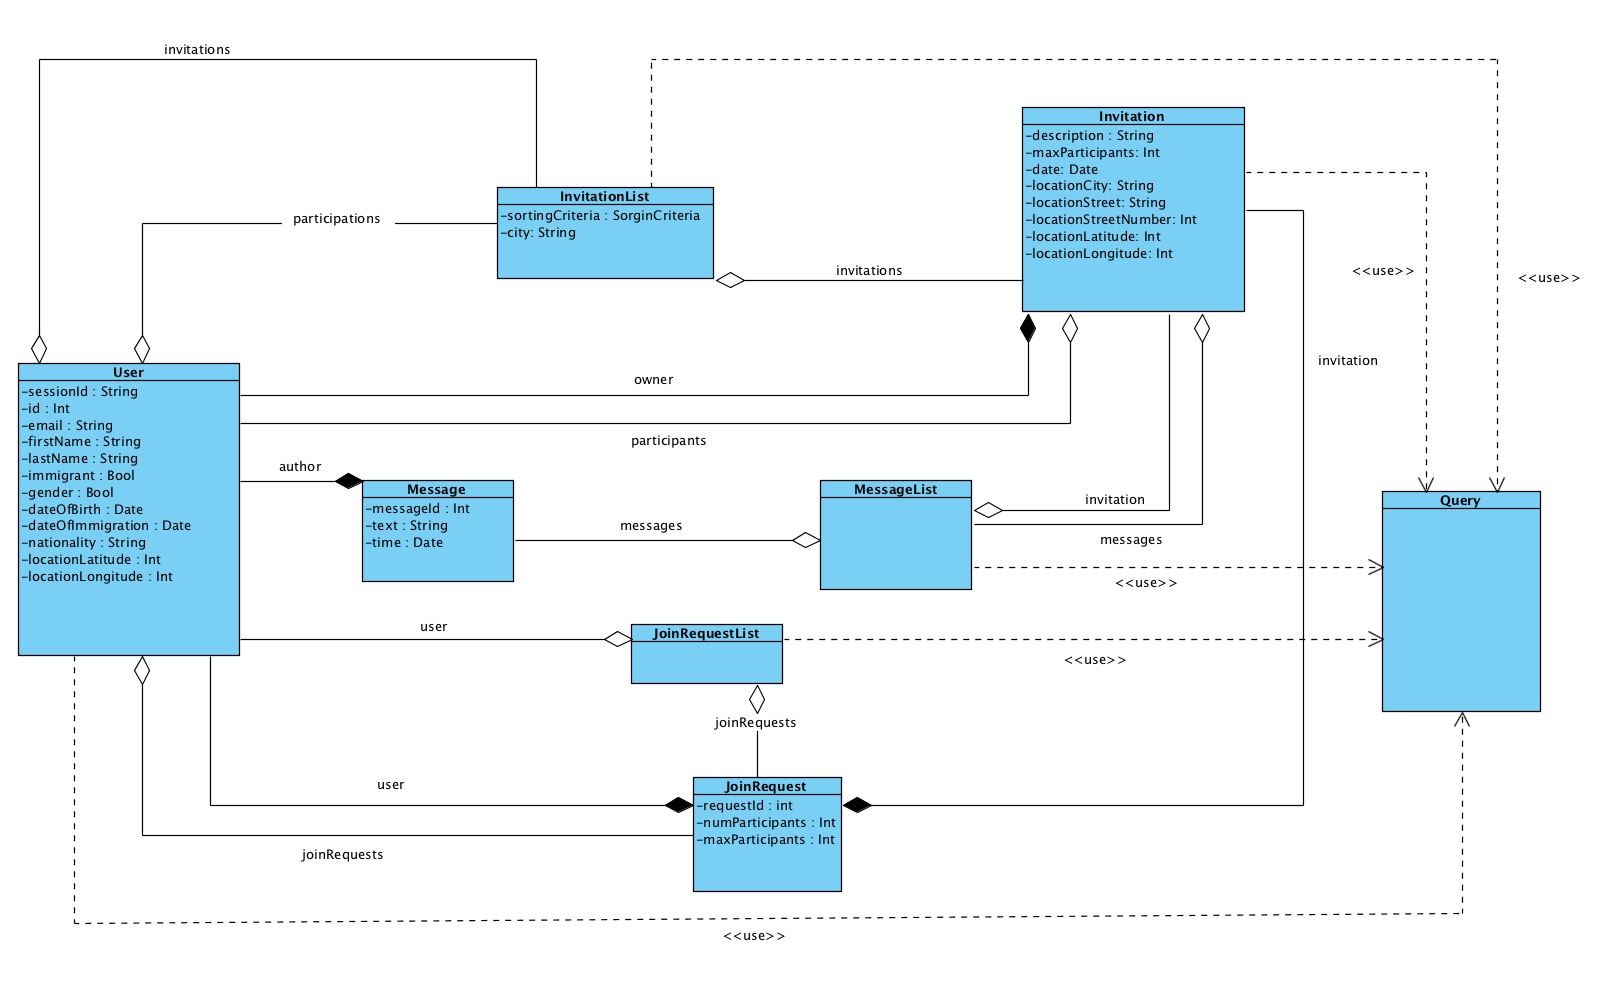
\includegraphics[width=0.9\textwidth]{../../spec/components/mobile_app_uml_class.png}
		\caption[UML class diagram of the mobile app model]{UML class diagram of the mobile app model}
		\label{fig:ios-class-diagram}
	\end{center}
\end{figure}

\newpage
List of \texttt{Query} subclasses:

\begin{itemize}
	\item for \texttt{User}
	\begin{itemize}
		\item \texttt{QueryUserDetail}
		\item \texttt{QueryUserLogin}
		\item \texttt{QueryUserLogout}
		\item \texttt{QueryUserRegister}
	\end{itemize}
	
	\item for \texttt{Invitation}
	\begin{itemize}
		\item \texttt{QueryInvitationList}
		\item \texttt{QueryInvitationCreate}
		\item \texttt{QueryInvitationJoin}
		\item \texttt{QueryInvitationUpdate}
		\item \texttt{QueryInvitationDelete}
		\item \texttt{QueryInvitationParticipants}
		\item \texttt{QueryInvitationDetail}
	\end{itemize}
	
	\item for \texttt{Message}
	\begin{itemize}
		\item \texttt{QueryMessagePost}
		\item \texttt{QueryMessageList}
	\end{itemize}
	
	\item for \texttt{JoinRequest}
	\begin{itemize}
		\item \texttt{QueryJoinRequestList}
		\item \texttt{QueryJoinRequestAccept}
		\item \texttt{QueryJoinRequestReject}
	\end{itemize}
	
\end{itemize}

\newpage
\subsection{iOS App}

The iOS user interface is built using \emph{Xcode} storyboards and based on wireframes in the specification. All UI classes are Apple \texttt{UIKit} subclasses like \texttt{UITableViewController} or \texttt{UITableViewCell}.\\
\\
The following points are considered for building a responsive iOS user interface:
\begin{itemize}
	\item The top level layout uses a \texttt{UITabBarController} which holds view controllers for top level functionality like displaying a list of invitations or the user profile
	
	\item \emph{Closures}: In most cases a view controller is querying resources over network. To not block the UI while waiting for a query to return, the queries are executed asynchronously. Therefore each method performing a network request has a \texttt{Void} return type and a \texttt{completion} handler that is executed when the request has returned.
	
	\item Since the completion handler runs on a different thread, UI elements cannot directly be updated but must be called again on the main thread using\\ \texttt{DispatchQueue.main.async \{...\}}.
	
	\item To ensure correct use of the \emph{Model View Controller} pattern no model logic must be executed in any view controller. Instead the view controller call methods of the model classes like \texttt{User} or \texttt{Invitation} and only displays the retrieved data.
\end{itemize}

\newpage
\subsection{Android app}

The user interface is built in Android Studio using \emph{XML} layout files, each view corresponds to a layout file. In code, the layouts are represented as \emph{Activies} or \emph{Fragments}, the corresponding Java classes are \texttt{AppCompatActivity} and \texttt{Fragment}. \\
\\
The following points are considered for building a responsive Android user interface:
\begin{itemize}
	\item The top level layout uses a \texttt{android.support.v4.widget.DrawerLayout} which holds a \texttt{fragment} for each top level functionality like displaying a list of invitations or the user profile
	
	\item \emph{Listeners}: In most cases a view controller is querying resources over network. To not block the UI while waiting for a query to return, the queries are executed asynchronously. In Android each method performing a network request defines a \texttt{Listener} which is an interface that the classes using the request must implement. The listener calls a completion method as soon as the network request returns.
	
\end{itemize}

\end{document}